\documentclass[handout,xcolor={usenames,dvipsnames},11pt]{beamer}

\defbeamertemplate{description item}{align left}{\insertdescriptionitem\hfill}

% \usetheme[sectionpage=none,subsectionpage=simple,progressbar=none,block=fill]{metropolis}
\usetheme[sectionpage=none,subsectionpage=simple,progressbar=frametitle,block=fill]{metropolis}
% \setsansfont[BoldFont={Fira Sans SemiBold}]{Fira Sans Book}
\usepackage{tikz}
\usetikzlibrary{patterns}
\usetikzlibrary{shapes.misc, positioning}
\usepackage{eso-pic}
\usepackage{booktabs}
\usepackage[scale=2]{ccicons}
\usepackage{pgfplots}
\usepackage{amsmath}
\usepackage{wasysym}
\usepackage{mathtools}
\usepackage{pgf}
\usepackage{pifont}
% \setsansfont{Ubuntu}
% \setmonofont{Ubuntu Mono}

\DeclarePairedDelimiter{\ceil}{\lceil}{\rceil}

\usepgfplotslibrary{dateplot}
\hypersetup{colorlinks,linkcolor=Cerulean,urlcolor=Cyan}

\usepackage{xspace}
\newcommand{\themename}{\textbf{\textsc{metropolis}}\xspace}
\usefonttheme[onlymath]{serif}
\setbeamertemplate{caption}{\raggedright\insertcaption\par}


\title{ \LARGE Turbo Codes for Deep Space Communications: CCSDS 131.0-B-2 standard implementation}
% \title{\LARGE Reccomendation for Space Data System Standards}
\subtitle{Final project for the Channel Coding course}
\author[G. Marcon]{Gianluca Marcon \hfill \href{mailto:gianluca.marcon.1@studenti.unipd.it}{gianluca.marcon.1@studenti.unipd.it}}
\date{\today}
% \institute{Department of Information Engineering, University of Padova}

% logo on every page
%\newcommand{\nologo}{\setbeamertemplate{logo}{}}

%\newcommand\AtPagemyUpperLeft[1]{\AtPageLowerLeft{%
%\put(\LenToUnit{0.94\paperwidth},\LenToUnit{0.03\paperheight}){#1}}}
%\AddToShipoutPictureFG{
%  \AtPagemyUpperLeft{{
\includegraphics[height=2cm,keepaspectratio]{./logos/DEI.png}}}
%}%

\logo{\vspace*{-1.4cm}
\includegraphics[height=2cm,keepaspectratio]{./logos/DEI.png}}


% full logo on title page
\titlegraphic{
\includegraphics[height=2cm]{./logos/unipd}\hfill
\includegraphics[height=2cm]{./logos/DEI_full}}
\setbeamertemplate{subsection page}[simple]

\begin{document}

\maketitle

%======================================================================================
\begin{frame}{Electro-optic modulators}
    Convert electronic signal to high bit-rate optical signal.\pause

    Desired features:\pause
    \begin{itemize}
        \item high switching speed\pause
        \item high bandwidth\pause
        \item small footprint (\emph{Nanoscale...})\pause
        \item compatibility with on-chip electronic components\pause
        \item low insertion loss\pause
        \item energy efficiency
    \end{itemize}    
    % Usually can't meet every requirement. 
\end{frame}
%======================================================================================
\begin{frame}{Graphene: why?}
    \vspace{10pt}
    \begin{minipage}{0.6\textwidth}
        \begin{figure}
            \centering
            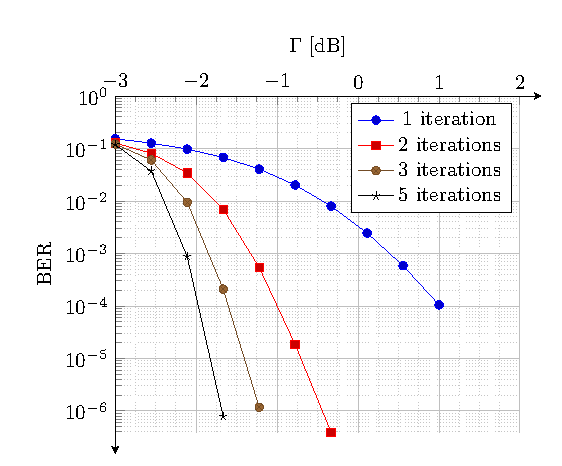
\includegraphics[width=\textwidth]{./images/BER}
        \end{figure}
    \end{minipage}\hfill
    \begin{minipage}{0.4\textwidth}
        \begin{itemize}
            \pause
            \item Flexible\pause
            \item Robust\pause
            \item Small footprint\pause
            \item Great thermal characteristics \pause
            \item \alert{High electron mobility}\pause
            \item \alert{\textbf{Voltage-dependent optical conductivity}}\pause
        \end{itemize}
    \end{minipage}
    \begin{center}
        \LARGE
        Great for high speed optical modulators!
    \end{center}
\end{frame}

%======================================================================================
\begin{frame}{However...}
    ...small dimensions of graphene can be a problem:\pause
    \begin{itemize}
        \item operating wavelength (1550 nm) is huge in comparison\pause
        \item need to enhance interaction with light\pause
        \item new waveguide designs must be studied
    \end{itemize}
    \begin{figure}
        \centering
        \begin{tikzpicture}
            \node (img3) {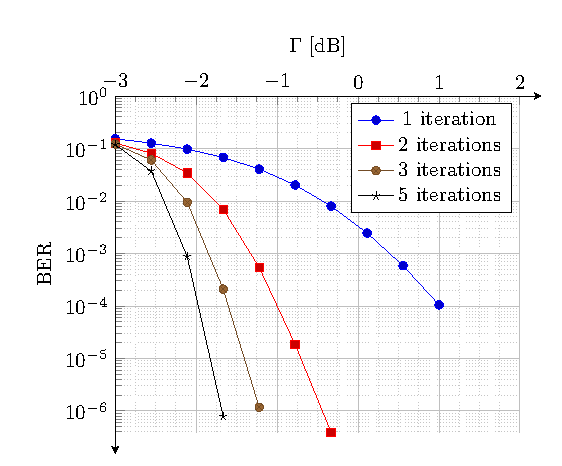
\includegraphics[height=3cm]{./images/BER}};
            \node (img4) at (img3.east)[xshift=2cm] {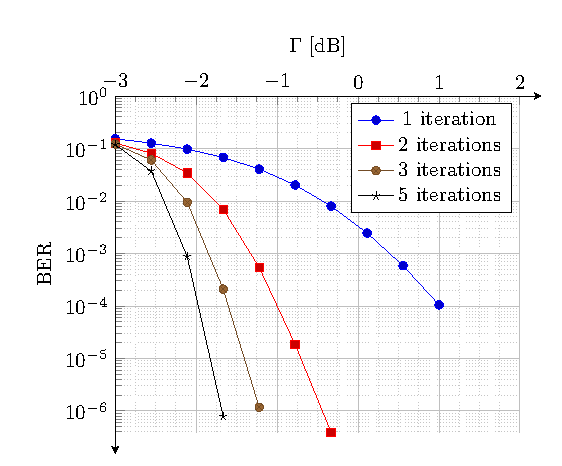
\includegraphics[height=3cm]{./images/BER}};
        \end{tikzpicture}
        \caption{\cite{Xu2004,Sun2007}}
    \end{figure}
\end{frame}

%======================================================================================
\begin{frame}{Light-graphene interaction}
    Two different phenomena:\pause
    \begin{itemize}
        \item \textbf{Interband absorption:} photon get absorbed and electron moves to conduction band\pause
        \item \textbf{Intraband absorption:} photon get absorbed and electron stays in same band but in a higher level\pause
    \end{itemize} 

    \begin{alertblock}{Conductivity}
        \vspace{-8pt}
        \begin{align*}
            \sigma_g &= \sigma_{inter}(\omega,\mu_c, T) + \sigma_{intra}(\omega,\mu_c, T) \\
                     &\simeq \sigma_{inter}(\omega,\mu_c, T)  
            \qquad\text{ when } \mu_c < \hbar\omega/2
        \end{align*}
    \end{alertblock} 
    %Both depend on chemical potential through applied \alert{gate voltage}.
\end{frame}

%======================================================================================
\begin{frame}[c]{Conductivity of graphene}
    \vspace{-15pt}
    \begin{figure}
        \centering
        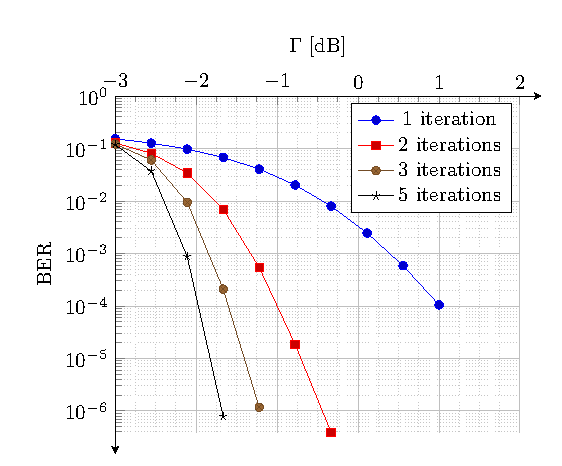
\includegraphics[height=\textheight]{./images/BER}
    \end{figure}\pause
\end{frame}

%======================================================================================
\begin{frame}[c]{First type of modulator}
    \begin{figure}
        \begin{center}
           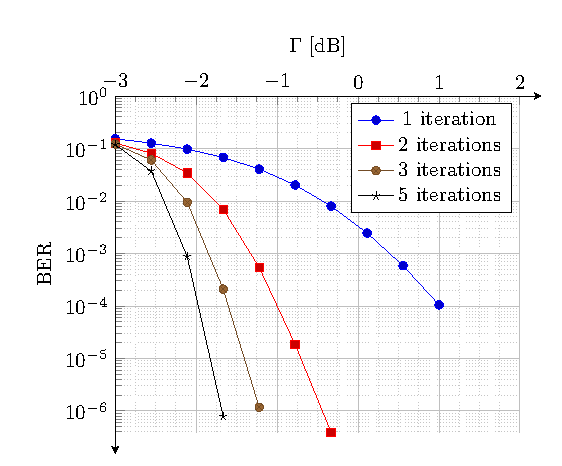
\includegraphics[width=0.6\textwidth]{./images/BER}
        \end{center}
        \caption{\cite{Cho2011}}
    \end{figure}\pause
    \begin{center}
        Large footprint required to obtain adequate modulation depth        
    \end{center}
\end{frame}
%======================================================================================
\begin{frame}[c]{Novel design: slot waveguides}
    \begin{figure}
        \centering
        \begin{tikzpicture}
            \node (img3) {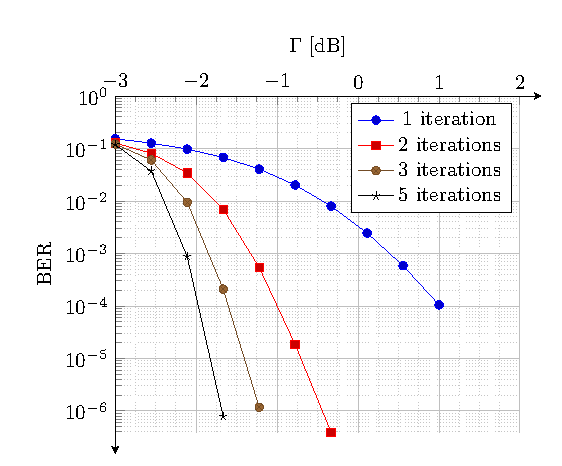
\includegraphics[height=3.5cm]{./images/BER}};
            \node (img4) at (img3.east)[xshift=2.5cm] {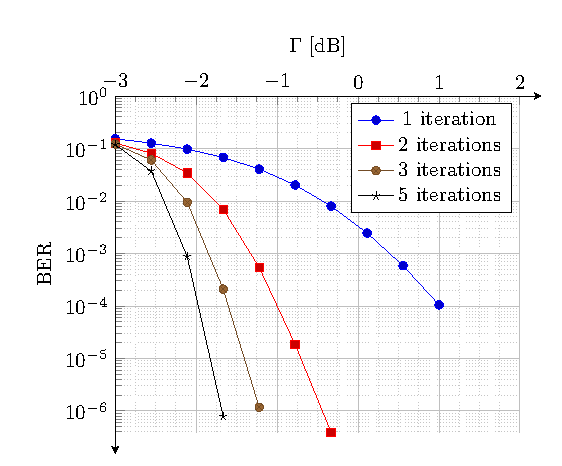
\includegraphics[height=3.5cm]{./images/BER}};
        \end{tikzpicture}
        \caption{$\lambda = 1550$ nm, $n_{co} = 1.46$, $n_{cl} = 3.48$, $w_{co} = 101$ nm. \cite{Xu2004}}
    \end{figure}\pause
    \begin{alertblock}{Absorbed power per unit area}
        \[
            P \propto \frac{1}{2} |\mathbf{E}| \cdot \frac{Im\{\varepsilon_{eff}\}}{|\varepsilon_{eff}|} 
        \]
    \end{alertblock}
\end{frame}  
%======================================================================================
\begin{frame}{Wavelength and Voltage dependency}
    \begin{figure}
        \centering
        \begin{tikzpicture}
            \node (img3) {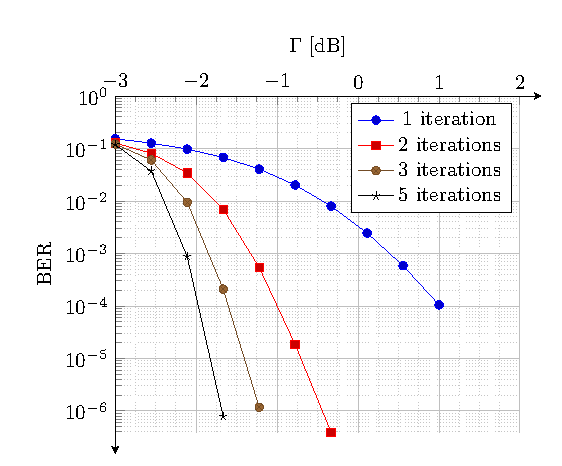
\includegraphics[height=4cm]{./images/BER}};
            \node (text1) at (img3.south)[yshift=-0.3cm]{Bandwidth > 1.25 THz};
            \node (img4) at (img3.east)[xshift=2.5cm] {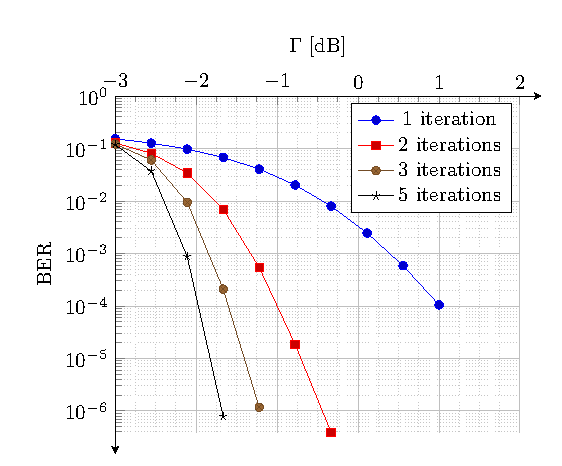
\includegraphics[height=4cm]{./images/BER}};
            \node (text2) at (img4.south)[yshift=-0.3cm]{$\Delta V = 1.32 V$};
        \end{tikzpicture}
    \end{figure}
    
\end{frame}
%======================================================================================
\begin{frame}[c]{Plasmonic-graphene waveguide modulator}
    \begin{figure}
        \centering
        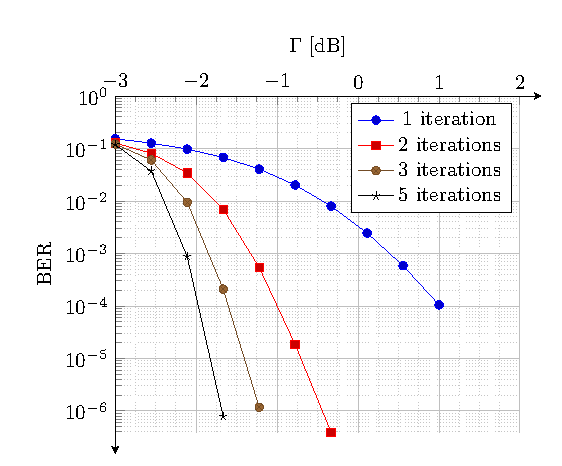
\includegraphics[height=4cm]{./images/BER}
    \end{figure}
    
    Cu is preferred (CMOS compatible), but has higher losses than Au, Ag.
\end{frame}
\begin{frame}{Plasmonic-graphene waveguide modulator}
    200 nm wide, silicone nitride 10 nm thick (both layers), length 120 nm.
    \begin{figure}
        \centering
        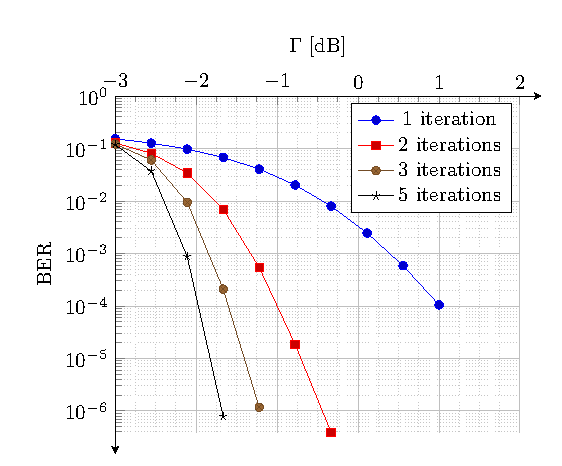
\includegraphics[width=0.5\textwidth]{./images/BER}
    \end{figure}    
    \begin{center}
        Footprint $ \sim 2-3 \;\mu m^2$
    \end{center}
\end{frame}
%======================================================================================
\begin{frame}{Wavelength and Voltage dependency}
    \begin{figure}
        \centering
        \begin{tikzpicture}
            \node (img3) {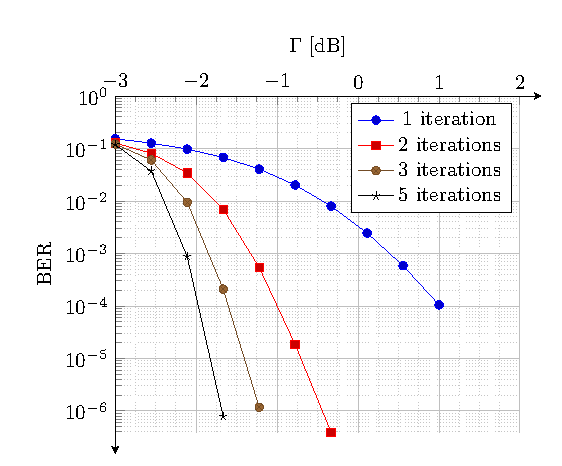
\includegraphics[height=4cm]{./images/BER}};
            \node (text1) at (img3.south)[yshift=-0.3cm]{Bandwidth > 1 THz};
            \node (img4) at (img3.east)[xshift=2.7cm] {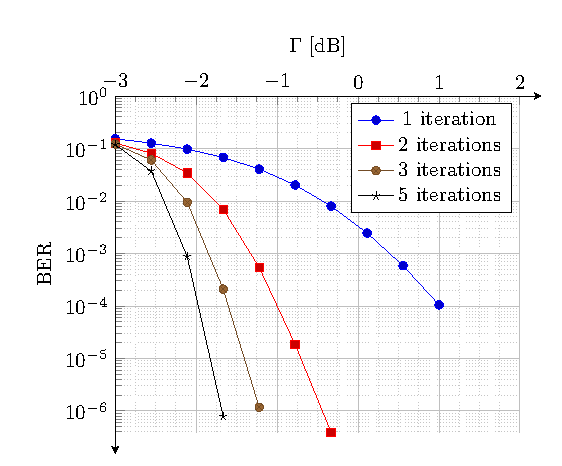
\includegraphics[height=4cm]{./images/BER}};
            \node (text2) at (img4.south)[yshift=-0.3cm]{$\Delta V = 1.38 V$};
        \end{tikzpicture}
    \end{figure}
    \begin{center}
        Energy consumption $\sim$ 0.12-0.13 pJ/bit
    \end{center}
\end{frame}
%======================================================================================
\begin{frame}{Did we meet any requirement?}
    \pause
    \begin{itemize}
        \item high bandwidth\pause\qquad \textcolor{TolLightGreen}{\textbf{Yes}}\pause
        \item energy efficiency\pause\qquad \textcolor{TolLightGreen}{\textbf{Yes}}\pause
    \item compatibility with on-chip electronic components\pause\quad \textcolor{TolLightGreen}{\textbf{Yes}}\pause
        \item low insertion loss\pause\qquad \textcolor{TolLightGreen}{\textbf{Yes}}\pause
        \item small footprint \pause\qquad \alert{\textbf{Kinda}} \pause
        \item high switching speed\pause\qquad \alert{\textbf{Potentially}}
    \end{itemize}
    % Usually can't meet every requirement. 
\end{frame}
%======================================================================================
\begin{frame}{Recent advances: graphene-on-silicon MZI}
    \begin{itemize}
        \item Fix one arm in "dielectric state" (low loss) of graphene
        \item Exploit changes in $Re\{ \varepsilon_{eff}\}$ wrt gate voltage to induce phase change
    \end{itemize}
    \begin{figure}
        \centering
        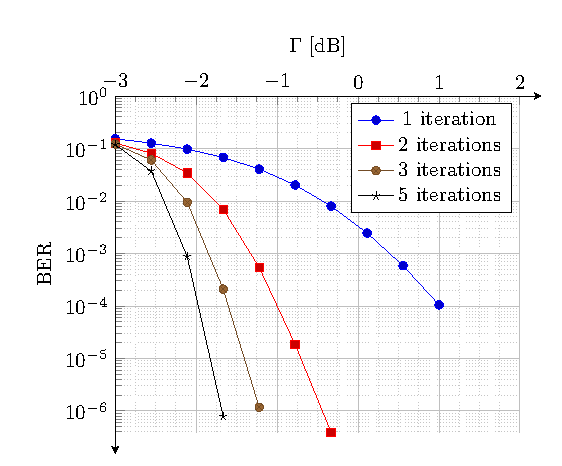
\includegraphics[width=0.5\textwidth]{./images/BER}
        \caption{\cite{Phatak2016}}
    \end{figure}
    %    Some references to showcase [allowframebreaks] \cite{knuth92,ConcreteMath,Simpson,Er01,greenwade93}
\end{frame}
%======================================================================================
\begin{frame}[standout]
    Thank you!
\end{frame}
%======================================================================================
\appendix

\begin{frame}[allowframebreaks]{References}

  \bibliography{demo}
  \bibliographystyle{apalike}

\end{frame}

\end{document}
